\documentclass[a4paper,11pt]{article}
\usepackage{a4wide}
\usepackage{fullpage}
\usepackage[utf8x]{inputenc}
\usepackage[toc,page]{appendix}
\usepackage[pdftex]{graphicx} % za slike
\usepackage{setspace}
\usepackage{color}
\usepackage{amsmath}
\usepackage{caption}
\usepackage{subcaption}
\usepackage{hyperref}
\definecolor{light-gray}{gray}{0.95}
\usepackage{hyperref}
\renewcommand{\baselinestretch}{1.2} % za boljšo berljivost večji razmak


\title{Linear classification}
\author{David Rubin (11917556)}
\date{\today}

\begin{document}

\maketitle

\section{Task summary}

We consider the data set \textit{vehicle.pkl}. The task is to classify a given silhouette as
one of two types of vehicles, i.e., SAAB or VAN, using a set of features extracted from
the silhouette. You are required to use Python for this assignment. The goal will be to
minimize misclassification rate on the test set. The data has been splitted into a training
set and a test set. First, extract from both of these sets only data points of the classes
SAAB ($C = 2$) and VAN ($C = 4$).

\section{Solution}

\subsection{Probabilistic generative model}

The code containing my solution for this approach is included in the file \textit{genmod.py}. When run, it should output a \textit{.CSV} file (called \textit{genmod.csv}) containing the raw accuracies for both the training and test set and for the numbers of features selected. It also outputs an image with the accuracy graph for different numbers of features. The graph is presented on figure~\ref{genmod:acc}. The model achieves its highest accuracy of $0.985$ on the training set when all features are used, and maintains an accuracy of $0.979$ when using 13 or more features on the test set. I did not check any combinations of features other than taking the first N from the given order. Results may vary if the features are chosen in different orders.

\begin{figure}
\centering
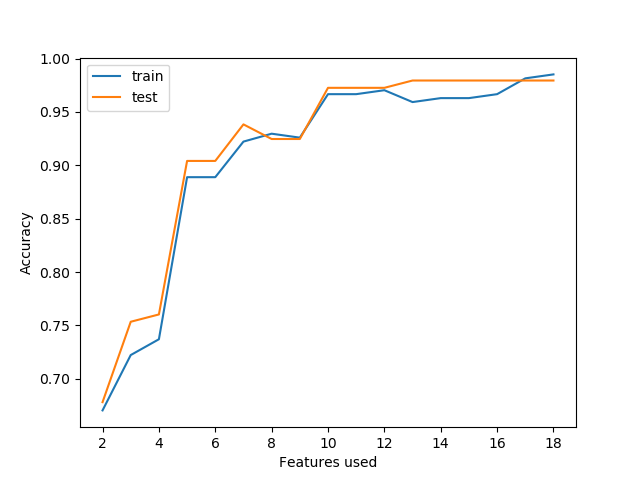
\includegraphics[width=0.8\textwidth]{images/genmod_acc.png}
\caption{The accuracy of my probabilistic generative model on both the training and test set for different numbers of features used.}
\label{genmod:acc}
\end{figure} 

\subsection{IRLS}

The code containing my solution for this approach is included in the file \textit{irls.py}. As in the first solution when running the code it produces a \textit{.CSV} file (called \textit{irls.csv}) and creates graphs for the misclassification rates and cross entropy errors during learning epochs for a different number of features used (specifically when 2, 9 or 18 features are used).

The initial weights are chosen as random numbers from $[-0.000001, 0.000001)$. For my solution I have introduced 3 stop conditions during the learning phase:
\begin{enumerate}
 \item \textit{maxiter} ... a maximum number of iterations which can occur (default 100)
 \item \textit{singularity} ... I check if the Hessian matrix is singular by computing the condition number of the matrix (2-norm) and checking is it is finite or not. On some occasions this test does not detect the singular matrix and the program returns an error when calculating the inverse. I have not found a better solution at the point of writing this report.
 \item \textit{Cross entropy error} ... as we will see later on the accuracy graph, I have gotten better results by stopping the learning process when the cross entropy error on the training set was low enough (rule of thumb stop when $CE_e<10^{-6}$). However I fear that this may cause overfitting the data, which on the given samples I haven't noticed.
\end{enumerate}
While on a low number of features, the stop condition of the max iterations was prevalent, while when a higher number of features were chosen the condition of a low cross entropy error stopped the learning at around 20-30 epochs.
The final accuracy of the model given 18 features was $0.959$ with a misclassification rate of $0.034$ on the test set and the test set cross entropy error of $+\infty$ on the last epoch. I am not sure what caused the last metric to rise to infinity, as it was declining in the first 6 epochs and then rose to infinity in the next 9. On the training set the cross entropy error kept declining and stayed in the rang of $10^{-7}$.

The graphs comparing the accuracy of my model with and without the cross entropy error stop condition are shown on figure~\ref{irls:acc}. The graphs showing the progression of the cross entropy errors are available on figure~\ref{irls:cee}. And finally the graphs for misclassification rates are presented on figure~\ref{irls:mcr}.

\begin{figure}
	\centering
	\begin{subfigure}[b]{0.49\textwidth}
		\centering
		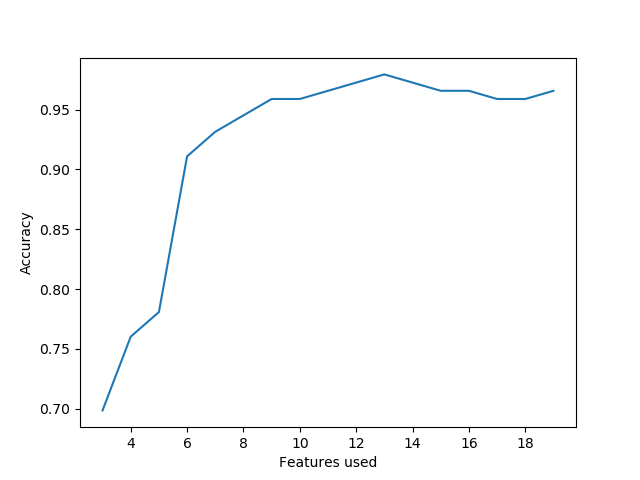
\includegraphics[width=\textwidth]{images/irls_acc.png}
		\caption{The accuracy on the test set given the limit with a low cross entropy error}
		\label{irls:acc_lim}
	\end{subfigure}
	\begin{subfigure}[b]{0.49\textwidth}
		\centering
		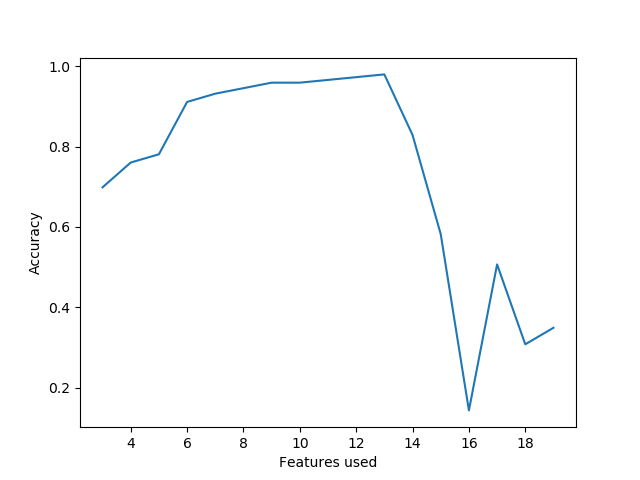
\includegraphics[width=\textwidth]{images/irls_acc2.png}
		\caption{The accuracy on the test set given limited by checking for a singularity in the matrix}
		\label{irls:acc_nolim}
	\end{subfigure}
	\caption{The accuracy of the model given a number of features and different limits.}
	\label{irls:acc}
\end{figure} 

\begin{figure}
	\centering
	\begin{subfigure}[b]{0.49\textwidth}
		\centering
		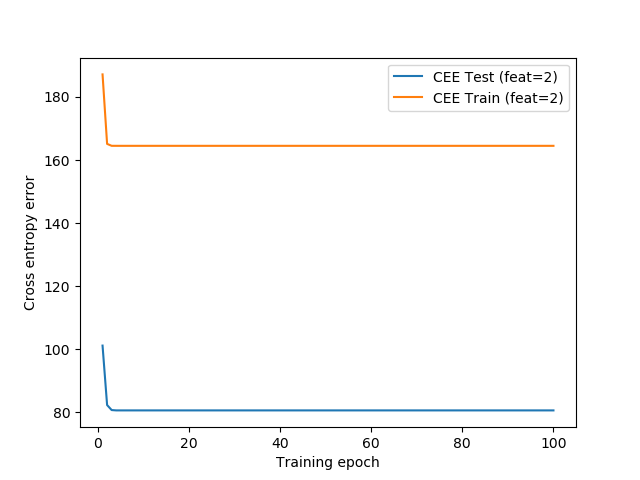
\includegraphics[width=\textwidth]{images/irls_cee-2.png}
		\caption{2 features are used}
		\label{irls:cee_2}
	\end{subfigure}
	\begin{subfigure}[b]{0.49\textwidth}
		\centering
		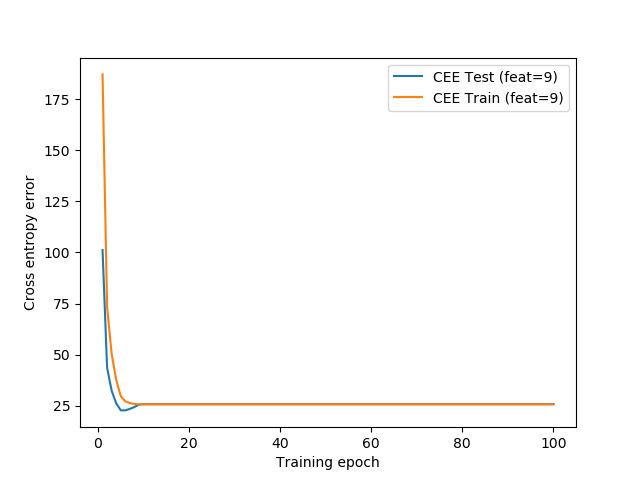
\includegraphics[width=\textwidth]{images/irls_cee-9.png}
		\caption{9 features are used}
		\label{irls:cee_9}
	\end{subfigure}
	\begin{subfigure}[b]{0.5\textwidth}
		\centering
		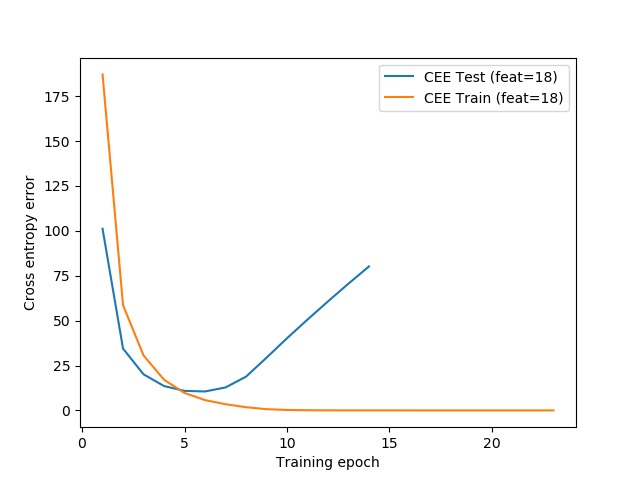
\includegraphics[width=\textwidth]{images/irls_cee-18.png}
		\caption{18 features are used. Note: on the test set the error rose to $+\infty$ after epoch 13}
		\label{irls:cee_18}
	\end{subfigure}
	\caption{The cross entropy errors during training for different numbers of features used.}
	\label{irls:cee}
\end{figure} 

\begin{figure}
	\centering
	\begin{subfigure}[b]{0.49\textwidth}
		\centering
		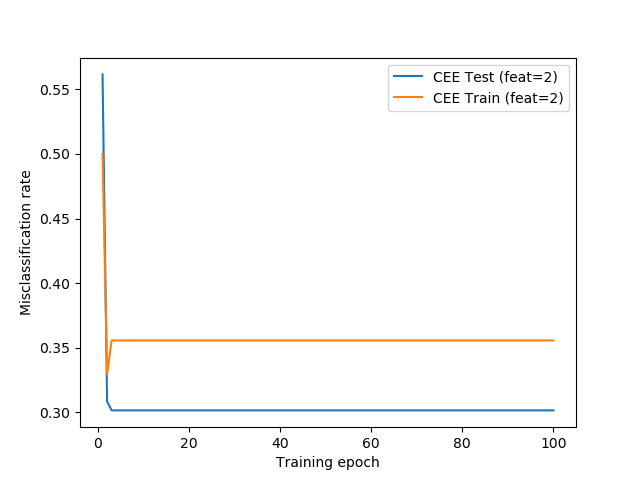
\includegraphics[width=\textwidth]{images/irls_mcr-2.png}
		\caption{2 features are used}
		\label{irls:mcr_2}
	\end{subfigure}
	\begin{subfigure}[b]{0.49\textwidth}
		\centering
		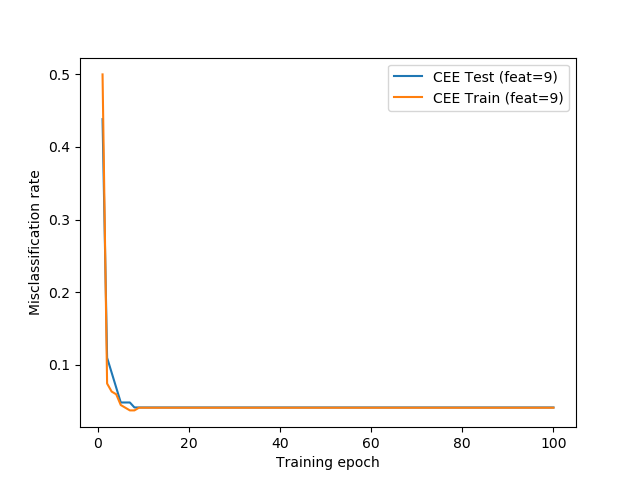
\includegraphics[width=\textwidth]{images/irls_mcr-9.png}
		\caption{9 features are used}
		\label{irls:mcr_9}
	\end{subfigure}
	\begin{subfigure}[b]{0.49\textwidth}
		\centering
		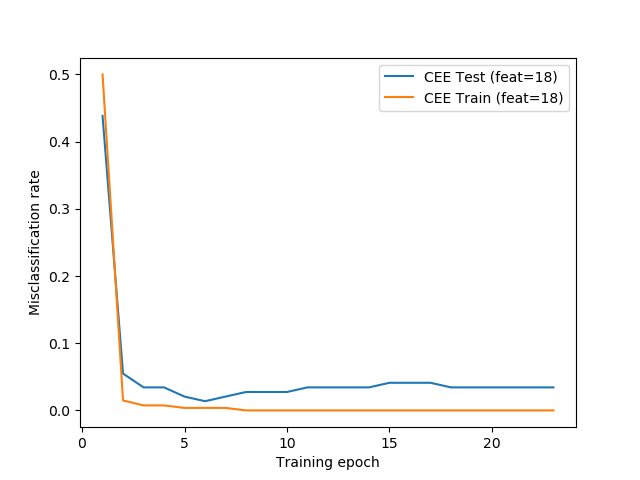
\includegraphics[width=\textwidth]{images/irls_mcr-18.png}
		\caption{18 features are used}
		\label{irls:mcr_18}
	\end{subfigure}
	\caption{The misclassification rate during training for different numbers of features used.}
	\label{irls:mcr}
\end{figure} 

\subsection{Comparison}

In terms of accuracy, my implementation of the probabilistic generative model achieved a better score on the test set ($0.979$ opposed to $0.959$ from IRLS) and from a programmers perspective it was much easier to implement. The uncertainty and possible problems arising when choosing initial weights for IRLS or deciding on its stop conditions seem to me that the method of a probabilistic generative approach is better-performing, atleast when using simple problems (as the one presented in this task). I have not tried to solve a more difficult task using both approaches and I can not say for sure that the easier implementation is better, but from what I have seen the \textit{KISS} approach\footnote{\url{https://en.wikipedia.org/wiki/KISS_principle}} seems to always be a valid option.
\end{document}
